\documentclass[10pt]{article}
\usepackage{amsmath}
\usepackage{geometry}
\usepackage{fancybox}
\usepackage{tikz}
\usepackage{listings}
 \geometry{
 a4paper,
 total={170mm,257mm},
 left=20mm,
 top=-5mm,
 bottom=15mm
 }
 
\usepackage{color}
 
\definecolor{codegreen}{rgb}{0,0.6,0}
\definecolor{codegray}{rgb}{0.5,0.5,0.5}
\definecolor{codepurple}{rgb}{0.58,0,0.82}
\definecolor{backcolour}{rgb}{0.95,0.95,0.92}

\linespread{1.3}

\title{CSC263H1 Assignment 3}
\author{Jiatao Xiang, Xu Wang, Huakun Shen}
\date{February 14th, 2019}

\begin{document}
\maketitle

\section*{Question 1}
\ovalbox{
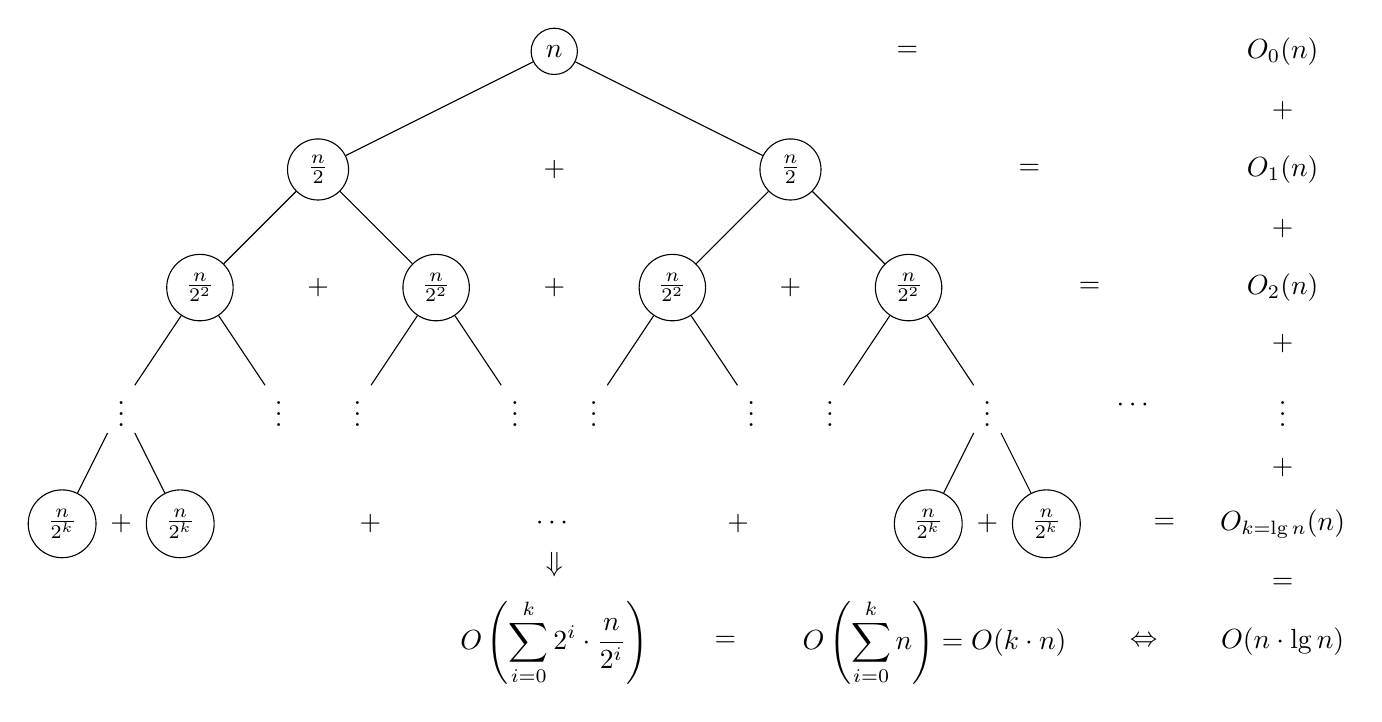
\begin{tikzpicture}[level/.style={sibling distance=60mm/#1}]
\node [circle,draw] (z){$n$}
  child {node [circle,draw] (a) {$\frac{n}{2}$}
    child {node [circle,draw] (b) {$\frac{n}{2^2}$}
      child {node {$\vdots$}
        child {node [circle,draw] (d) {$\frac{n}{2^k}$}}
        child {node [circle,draw] (e) {$\frac{n}{2^k}$}}
      } 
      child {node {$\vdots$}}
    }
    child {node [circle,draw] (g) {$\frac{n}{2^2}$}
      child {node {$\vdots$}}
      child {node {$\vdots$}}
    }
  }
  child {node [circle,draw] (j) {$\frac{n}{2}$}
    child {node [circle,draw] (k) {$\frac{n}{2^2}$}
      child {node {$\vdots$}}
      child {node {$\vdots$}}
    }
  child {node [circle,draw] (l) {$\frac{n}{2^2}$}
    child {node {$\vdots$}}
    child {node (c){$\vdots$}
      child {node [circle,draw] (o) {$\frac{n}{2^k}$}}
      child {node [circle,draw] (p) {$\frac{n}{2^k}$}
        child [grow=right] {node (q) {$=$} edge from parent[draw=none]
          child [grow=right] {node (q) {$O_{k = \lg n}(n)$} edge from parent[draw=none]
            child [grow=up] {node (r) {$\vdots$} edge from parent[draw=none]
              child [grow=up] {node (s) {$O_2(n)$} edge from parent[draw=none]
                child [grow=up] {node (t) {$O_1(n)$} edge from parent[draw=none]
                  child [grow=up] {node (u) {$O_0(n)$} edge from parent[draw=none]}
                }
              }
            }
            child [grow=down] {node (v) {$O(n \cdot \lg n)$}edge from parent[draw=none]}
          }
        }
      }
    }
  }
};
\path (a) -- (j) node [midway] {+};
\path (b) -- (g) node [midway] {+};
\path (k) -- (l) node [midway] {+};
\path (k) -- (g) node [midway] {+};
\path (d) -- (e) node [midway] {+};
\path (o) -- (p) node [midway] {+};
\path (o) -- (e) node (x) [midway] {$\cdots$}
  child [grow=down] {
    node (y) {$O\left(\displaystyle\sum_{i = 0}^k 2^i \cdot \frac{n}{2^i}\right)$}
    edge from parent[draw=none]
  };
\path (q) -- (r) node [midway] {+};
\path (s) -- (r) node [midway] {+};
\path (s) -- (t) node [midway] {+};
\path (s) -- (l) node [midway] {=};
\path (t) -- (u) node [midway] {+};
\path (z) -- (u) node [midway] {=};
\path (j) -- (t) node [midway] {=};
\path (y) -- (x) node [midway] {$\Downarrow$};
\path (v) -- (y)
  node (w) [midway] {$O\left(\displaystyle\sum_{i = 0}^k n\right) = O(k \cdot n)$};
\path (q) -- (v) node [midway] {=};
\path (e) -- (x) node [midway] {+};
\path (o) -- (x) node [midway] {+};
\path (y) -- (w) node [midway] {$=$};
\path (v) -- (w) node [midway] {$\Leftrightarrow$};
\path (r) -- (c) node [midway] {$\cdots$};
\end{tikzpicture}}

\section*{Question 2}

\lstdefinestyle{mystyle}{
    backgroundcolor=\color{backcolour},   
    commentstyle=\color{codegreen},
    keywordstyle=\color{magenta},
    numberstyle=\tiny\color{codegray},
    stringstyle=\color{codepurple},
    basicstyle=\footnotesize,
    breakatwhitespace=false,         
    breaklines=true,                 
    captionpos=b,                    
    keepspaces=true,                 
    numbers=left,                    
    numbersep=5pt,                  
    showspaces=false,                
    showstringspaces=false,
    showtabs=false,                  
    tabsize=2
}
\lstset{style=mystyle}
\section*{Question 3}
\begin{enumerate}
\item[a.] Our data structure is based on \textbf{hash table}.\\
\textbf{Idea:} Put every element of set \textbf{B} into a hash table. Then hash every element of set \textbf{A} to a
slot in the hash table, and check whether the element of \textbf{A} is in this slot. If it is not in the slot, then it means that the element of set \textbf{A} is not in set \textbf{B}.\\
\textbf{Pseudo Code:}\\
Suppose \textbf{$\alpha$ = 10}, that is, each slot contains a linked list with size of at most approximately 10 elements.\\
Suppose we have a hash table \textbf{\textit{T}} with a size of $\frac{n}{\alpha}$.\\
Suppose we have a hashing function \textit{\textbf{h(x)}} that would return the index of one of the slots of \textbf{T} given \textbf{\textit{x}} as a input. Also assume \textbf{SUHA}.
\begin{lstlisting}[language=Python]
def h(x, num_slot):
	return x % num_slot
\end{lstlisting}
\begin{lstlisting}[language=Python]
for element in B:
		linked_list = T[h(element, len(T))]
		linked_list.append(element)
		
result = []
for element in A:
		linked_list = T[h(element, len(T))]
		for item in linked_list:
				if element == item:
						break
		result.append(element)
\end{lstlisting}
\item[b.]
Assumptions:\
\begin{itemize}
\item The linked list in each slot of hash table has approximately a length of $\alpha$ = 10
\item Hash table \textbf{T} has a length of $\frac{len(A)}{\alpha}$
\item SUHA for hash function \textbf{\textit{h(x, num\_slot)}}
\end{itemize}
Explanation:
Part I: put \textbf{B} into \textbf{T}
\begin{enumerate}
\item[1.] Hashing function costs constant time
\item[2.] There are $n$ elements in \textbf{B}, performing hashing function \textbf{\textit{h}} for each element of \textbf{B} costs $\mathcal{O}(n\times1)$ of time.
\end{enumerate}
Part II: match element of \textbf{A} to \textbf{T}
\begin{enumerate}
\item[1.] Each linked list in each slot of \textbf{T} has a size of at most $\alpha$ (by \textbf{SUHA}), which is constant. In the worst case, we have to traverse through every linked list, which costs $\mathcal{O}(\alpha)=\mathcal{O}(1)$ of time.
\item[2.] There are $n$ elements in \textbf{A}, performing step 1 for each of them costs $\mathcal{O}(\alpha n)=\mathcal{O}(n)$ of time.
\end{enumerate}
\item[c.]
\end{enumerate}


\end{document}
